\documentclass{article}
\usepackage{graphicx} % Required for inserting images
\usepackage{float}
\usepackage{amsmath}

\title{Compute Intelligence PS s7 Lab 1}
\author{Joris Plaščinskas}
\date{September 2024}


\begin{document}
    \maketitle
    \section{Introduction}
        The goal of this exercise is to explore what a virtual neuron is and find it's parameter values $\vec{W}$ and b that fit the given data. The parameter values should be found both using software and by solving mathematical equations. For this (and probably all other) labs I chose to use python for doing digital computations.
    \section{Code Overview}
        I started by defining what a neuron is and the possible activation functions it can have. The neuron function is defined using linear algebra, so it's input is: $\mathbf{X}$ a matrix of shape: $2 \times 4$ (feature count $\times$ data point count) and $\vec{W}$ a horizontal vector of feature count length.
        \begin{figure}[H]
            \centering
            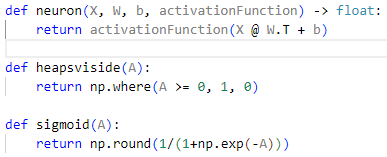
\includegraphics[width=0.8\textwidth]{ml.png}
            \caption{Neuron and it's activation functions}
            \label{fig:ml}
        \end{figure}
    
        The parameter search happens inside the code block seen in the Figure~\ref{fig:param}. The upper part is the random search and the lower is the iterative search. The iterative search takes many times longer to find suitable $\vec{W}$ and b values that fit $\mathbf{X}$ and $\vec{Y}$. Iterative search essentially goes through all the possible combinations of $w_0$,$w_1$ and b in increments of 5 until it finds 5 solutions. The random search just generates random: $w_0$,$w_1$ and b until it finds 5 solutions.
        \begin{figure}[H]
            \centering
            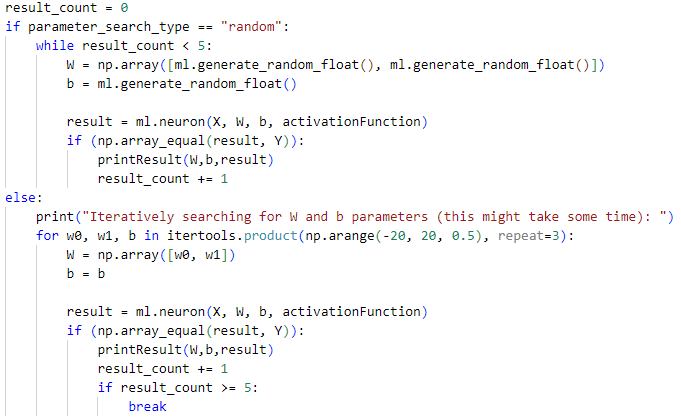
\includegraphics[width=1\textwidth]{parameter-search.png}
            \caption{Finding $\vec{W}$ and b}
            \label{fig:param}
        \end{figure}
    \section{Results Using Software}
        \begin{table}[H]
        \centering
        \caption{Data points}
        \begin{tabular}{|c|c|c|}
        \hline
        \multicolumn{2}{|c|}{$\mathbf{X}$} & $\vec{Y}$ \\
        \hline
        $x_{1}$ & $x_{2}$ & t \\
        \hline
        -0,2 & 0,5 & 0 \\
        \hline
        0,2 & -0,7 & 0 \\
        \hline
        0,8 & -0,8 & 1 \\
        \hline
        0,8 & 1 & 1 \\
        \hline
        \end{tabular}
        \end{table}
        
        \begin{table}[H]
        \centering
        \caption{Iterative, Sigmoid (old)}
        \begin{tabular}{|c|c|c|}
        \hline
        $w_{1}$ & $w_{2}$ & b\\
        \hline
        -5,5 & 19,5 & -11 \\
        \hline
        -5 & 17 & -9,5 \\
        \hline
        -5 & 18 & -10 \\
        \hline
        -5 & 18,5 & -10,5 \\
        \hline
        -5 & 19 & -11 \\
        \hline
        \end{tabular}
        \end{table}

        \begin{table}[H]
        \centering
        \caption{Iterative, Heapsviside}
        \begin{tabular}{|c|c|c|}
        \hline
        $w_{1}$ & $w_{2}$ & b\\
        \hline
        -5,5 & 19,5 & -11 \\
        \hline
        -5 & 17,5 & -10 \\
        \hline
        -5 & 18,5 & -10,5 \\
        \hline
        -5 & 19 & -11 \\
        \hline
        -5 & 19,5 & -11,5 \\
        \hline
        \end{tabular}
        \end{table}

        \begin{table}[H]
        \centering
        \caption{Random, Sigmoid}
        \begin{tabular}{|c|c|c|}
        \hline
        $w_{1}$ & $w_{2}$ & b\\
        \hline
        11,3 & 11 & -11,6 \\
        \hline
        11,3 & 7,2 & -14,7 \\
        \hline
        8 & 5,4 & -3,8 \\
        \hline
        12,2 & 6,2 & -10,8 \\
        \hline
        6,8 & 15,3 & -14,6 \\
        \hline
        \end{tabular}
        \end{table}

        \begin{table}[H]
        \centering
        \caption{Random, Heapsviside}
        \begin{tabular}{|c|c|c|}
        \hline
        $w_{1}$ & $w_{2}$ & b\\
        \hline
        11,1 & 18,2 & -16,6 \\
        \hline
        15,8 & 7,2 & -7,9 \\
        \hline
        14,7 & -2,5 & -8,5 \\
        \hline
        8,8 & 3,3 & -6,6 \\
        \hline
        16,9 & -4,1 & -6,4 \\
        \hline
        \end{tabular}
        \end{table}

        For the most part I expected such results. But I didn't expect the Iterative Sigmoid to differ from Iterative, Heapsviside. Because a rounded version of Sigmoid should essentially be the same function as Heapsviside. After some debugging and with the help of an LLM:) I managed to figure out that np.round(0.5) = 0. After fixing this issue with other rounding method the results of rounded Sigmoid became identical to Heapsviside.
    \section{Finding $\vec{W}$ and b Mathematically}
        \begin{math}
            He(\mathbf{X}W^{T}+b)=\vec{Y}\\
            \\
            He\left(
            \begin{bmatrix}
                x_{11}w_{1} + x_{12}w_{2} + b \\
                x_{21}w_{1} + x_{22}w_{2} + b \\
                x_{31}w_{1} + x_{32}w_{2} + b \\
                x_{41}w_{1} + x_{42}w_{2} + b
            \end{bmatrix}
            \right) = 
                \begin{bmatrix}
                y_1 \\
                y_2 \\
                y_3 \\
                y_4
            \end{bmatrix}
            \\
            \\
          He\left(
            \begin{bmatrix}
                -0,2w_{1} + 0,5w_{2} + b \\
                0,2w_{1} + -0,7w_{2} + b \\
                0,8w_{1} + -0,8w_{2} + b \\
                0,8w_{1} + 1w_{2} + b
            \end{bmatrix}
            \right) = 
                \begin{bmatrix}
                0 \\
                0 \\
                1 \\
                1
            \end{bmatrix}
            \\
            \\
            \\
            \begin{bmatrix}
                He(-0,2w_{1} + 0,5w_{2} + b) \\
                He(0,2w_{1} + -0,7w_{2} + b) \\
                He(0,8w_{1} + -0,8w_{2} + b) \\
                He(0,8w_{1} + 1w_{2} + b)
            \end{bmatrix}
            = 
                \begin{bmatrix}
                0 \\
                0 \\
                1 \\
                1
            \end{bmatrix}
            \\
            \\
            \\
            \begin{cases}
            He(-0,2w_{1} + 0,5w_{2} + b) &= 0 \\
            He(0,2w_{1} + -0,7w_{2} + b) &= 0 \\
            He(0,8w_{1} + -0,8w_{2} + b) &= 1 \\
            He(0,8w_{1} + 1w_{2} + b) &= 1 \\
            \end{cases}
            \\
            \\
            \\
            \begin{cases}
            -0,2w_{1} + 0,5w_{2} + b &< 0 \\
            0,2w_{1} + -0,7w_{2} + b &< 0 \\
            0,8w_{1} + -0,8w_{2} + b &>= 0 \\
            0,8w_{1} + 1w_{2} + b &>= 0 \\
            \end{cases}
        \end{math}
        
        \begin{figure}[H]
            \centering
            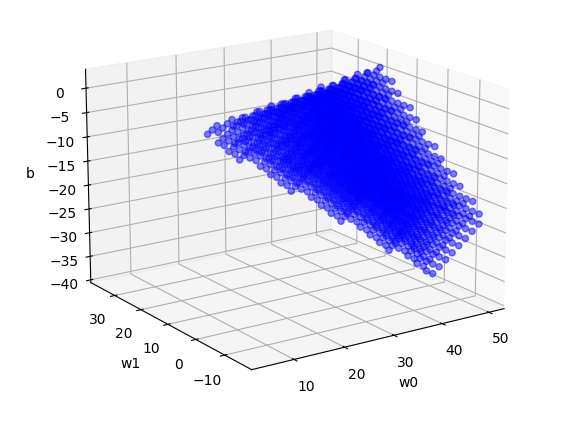
\includegraphics[width=0.8\textwidth]{solution-space.png}
            \caption{Solution space}
            \label{fig:ml}
        \end{figure}

        \begin{math}
            \begin{cases}
            -0,2*30 + 0,5*10 - 10 &< 0 \\
            0,2*30 + -0,7*10 - 10 &< 0 \\
            0,8*30 + -0,8*10 - 10 &>= 0 \\
            0,8*30 + 1*10 - 10 &>= 0 \\
            \end{cases}
        \end{math}
        \\
        \\
        The correctness of the above equation system was tested by substituting point a point from the graph: $w_0=30,w_1=10,b=-10$.
    \section{Conclusion}
        During this lab we learned that a neuron is just a set of parameters $\vec{w}$, b and an activation function. The neuron is essentially a function that is built using these parameters and the activation function. The input of this function is a vector or a matrix $\mathbf{X}$ and the output is the activation value/vector. Also by plotting, we learned that the parameter space that fits all data points is very big (infinite).
\end{document}
